\documentclass[portrait,plainboxedsections]{sciposter}

% Select Computer Concrete as default font
\usepackage{anyfontsize}
\usepackage{concrete}
\usepackage{concmath}
\usepackage{type1ec}
\usepackage[T1]{fontenc}
\renewcommand{\familydefault}{\rmdefault}


\usepackage{natbib}
\usepackage{amsmath}
\usepackage{amssymb}
\usepackage{booktabs}
\usepackage{graphicx}
%\usepackage{aas_macros}
\newcommand{\prd}{Phys. Rev. D}
\usepackage{xcolor}

\newcommand{\earlywarning}{early-warning}
\newcommand{\GW}{{\sc gw}}
\newcommand{\EM}{{\sc em}}
\newcommand{\GRB}{{\sc grb}}
\newcommand{\CBC}{{\sc cbc}}
\newcommand{\LIGO}{{\sc ligo}}
\newcommand{\LCGT}{{\sc lcgt}}
\newcommand{\GEO}{{\sc geo600}}
\newcommand{\ISCO}{{\sc isco}}
\newcommand{\SNR}{{\sc snr}}
\newcommand{\realtime}{real-time}
\newcommand{\Msun}{\ensuremath{M_{\odot}}}
\newcommand{\order}[1]{\ensuremath{\mathcal{O}[#1]}}
\newcommand{\tmpsamps}{\ensuremath{N}}
\newcommand{\numtmps}{\ensuremath{M}}
\newcommand{\numslices}{\ensuremath{S}}
% macros for number of svd basis functions
\newcommand{\SVD}{{\sc svd}}
\newcommand{\svdtmps}[1]{\ensuremath{L^#1}}
\newcommand{\numsvdtmps}{\svdtmps{s}}
% macros for sample points in slices
\newcommand{\slicesamps}[1]{\ensuremath{N^#1}}
\newcommand{\slicessamps}{\slicesamps{s}}
\newcommand{\fftblock}{\ensuremath{D}}
\newcommand{\resampsamps}{\ensuremath{N^\shortdownarrow,\, N^\shortuparrow}}
\newcommand{\fir}{{\sc fir}}
\newcommand{\fft}{{\sc fft}}
\newcommand{\fmax}{\ensuremath{f^0}}
\newcommand{\flops}{flop/s}
\newcommand{\gstlal}{{\tt gstlal}}
\newcommand{\gstreamer}{{\tt GStreamer}}
\newcommand{\numcpus}{{600}}
\newcommand{\lloid}{{\sc lloid}}
\newcommand{\TD}{{\sc td}}
\newcommand{\FD}{{\sc fd}}

% Macros for collapsing sizes of things
% From TUGboat, Volume 22 (2001), No. 4
% http://www.tug.org/TUGboat/tb22-4/tb72perlS.pdf
\def\clap#1{\hbox to 0pt{\hss#1\hss}}
\def\mathllap{\mathpalette\mathllapinternal}
\def\mathrlap{\mathpalette\mathrlapinternal}
\def\mathclap{\mathpalette\mathclapinternal}
\def\mathllapinternal#1#2{\llap{$\mathsurround=0pt#1{#2}$}} 
\def\mathrlapinternal#1#2{\rlap{$\mathsurround=0pt#1{#2}$}} 
\def\mathclapinternal#1#2{\clap{$\mathsurround=0pt#1{#2}$}}

% Colors for signal flow diagram and equation
\def\diagramcolorfir{red}
\def\diagramcolorreconstruct{blue}
\def\diagramcoloraccum{red!50!yellow}

% customize colors
\definecolor{BoxCol}{RGB}{0,35,102} % RoyalBlue
\definecolor{SectionCol}{RGB}{255,255,255} % White

\title{Toward early-warning detection of compact binary coalescence}

\author{\textsc{Nickolas V. Fotopoulos}, Leo P. Singer}

\institute{\LIGO{} Laboratory, California Institute of Technology}

\email{foton@caltech.edu}

\renewcommand{\sPlainBoxSection}[1]{
  \vspace{\secskip}
    \setlength{\secboxwidth}{\columnwidth}
    \addtolength{\secboxwidth}{-1cm}
    \setlength{\fboxrule}{2pt}
    \setlength{\fboxsep}{0pt}
        \vspace{1.1ex}
          \hspace{1.1ex}{\sectionsize{#1}} \\
  \rule[10pt]{\textwidth}{2pt}
  \par\vspace{1ex}
}


\begin{document}
%\conference{Amaldi 9, Cardiff, Wales, UK; This document bears the \textsc{dcc} number \LIGO{}-\textsc{g}\oldstylenums{1100683}-v\oldstylenums{1}.}

\begin{minipage}[b]{0.25\textwidth}
\raggedleft
{\fontsize{36}{50}\selectfont
Poster presented by

NF --- foton@caltech.edu

and LS --- lsinger@caltech.edu

}
\vspace{32mm}
\PARstart{}{Be sure to read article in preparation}

\fontsize{36}{40}\selectfont
arXiv:xxxx.xxxx
\end{minipage}%
\hspace{0.05\textwidth}%
\begin{minipage}[b]{0.6\textwidth}
{\fontsize{80}{100}\selectfont%
Toward early-warning detection

of compact binary coalescence

\vspace{0.5em}
\fontsize{30}{40}\selectfont
	Kipp Cannon,
	Romain Cariou,
	Adrian Chapman,
	Mireia Crispin-Ortuzar,
	Nickolas Fotopoulos,
	Melissa Frei,
	Chad Hanna,
	Erin Kara,
	Drew Keppel,
	Laura Liao,
	Stephen Privitera,
	Antony Searle,
	Leo Singer, and
	Alan Weinstein

%\vspace{0.5em}
%LIGO Laboratory, California Institute of Technology
}
\end{minipage}
\vspace{1cm}


\begin{minipage}[t]{0.25\textwidth}

\section*{Motivation}
\PARstart{\color{ink1!50!black}A}{\color{ink1!50!black}s a compact binary system} loses energy to gravitational waves (\GW{}s), its
orbital separation decays, leading to a runaway inspiral with the \GW{}
amplitude and frequency increasing until the system eventually merges.  If a
neutron star (\textsc{ns}) is involved, it may become tidally disrupted near
the merger and fuel an electromagnetic (\EM{}) counterpart~%
\citep{shibata:2007}.  Effort from both the \GW{} and astronomy communities may make it
possible to use \GW{} observations as an early warning trigger for \EM{}
followup.
%
\begin{figure}[h]
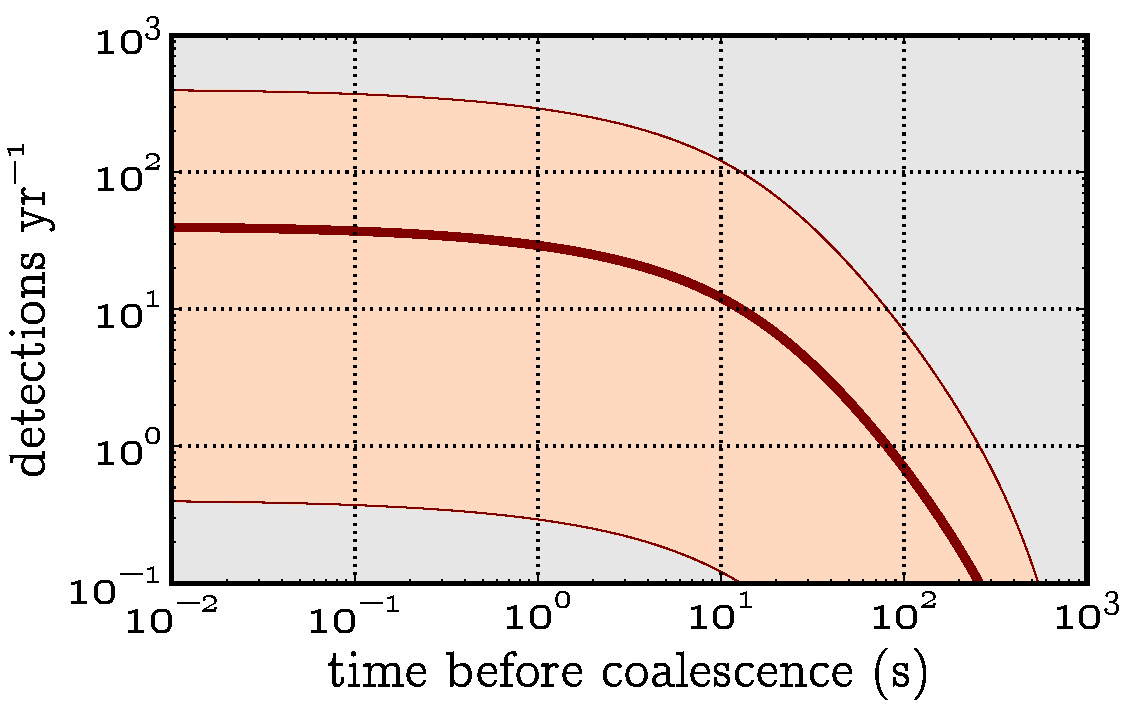
\includegraphics[width=1.05\textwidth]{figures/snr_in_time}
\caption{\label{fig:earlywarning}Expected number of \textsc{ns}--\textsc{ns}
sources that could be detectable by Advanced \LIGO\ a given number of seconds
before coalescence.  The heavy solid line is the most realistic yearly rate
estimate.  The shaded region represents the 5 to 95\% confidence interval
arising from uncertainty in predicted event rates~\citep{Abadie:2010p10836}.}
\end{figure}

\begin{figure}[h]
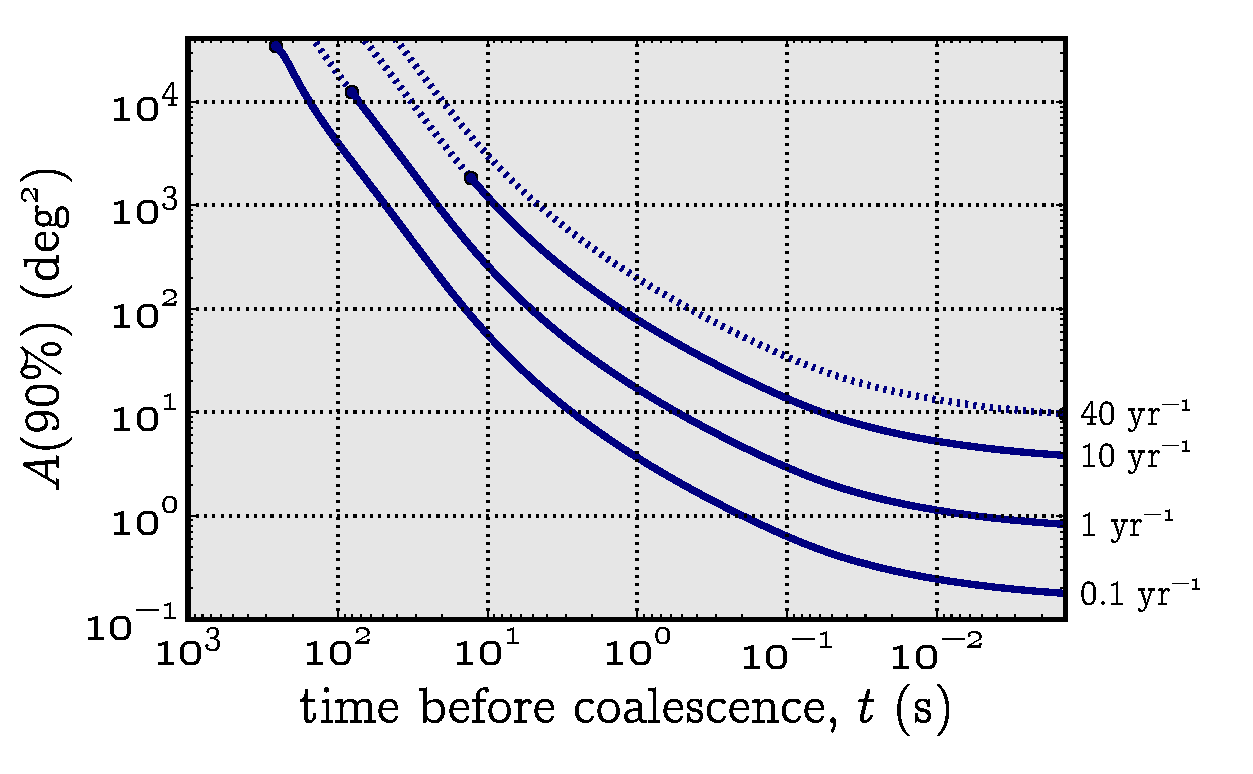
\includegraphics[width=1.15\textwidth]{figures/loc_in_time}
\caption{\label{fig:sky-localization-accuracy}Area of the 90\% confidence
region~\citep{Fairhurst2009} as a function of time before coalescence for sources with anticipated
detectability rates of 40, 10, 1, and 0.1~yr$^{-1}$. The heavy dot indicates
the time at which the accumulated \SNR\ exceeds a threshold of~8.}
\end{figure}

There were a number of sources of latency associated with the search for
\CBC{} signals in S6/VSR3~\citep{HugheyGWPAW2011}:

\begin{itemize}
\item Data acquisition and aggregation ($\gtrsim$100~ms)

\item Data conditioning ($\sim$1~min)

\item Trigger generation (2--5~min)

\item Alert generation (2--3~min)

\item Human validation (10--20~min)

\end{itemize}

\end{minipage}%
\hspace{0.05\textwidth}%
\begin{minipage}[t]{0.4\textwidth}

\section*{The LLOID algorithm}

\begin{figure}[h!]
	\begin{center}
		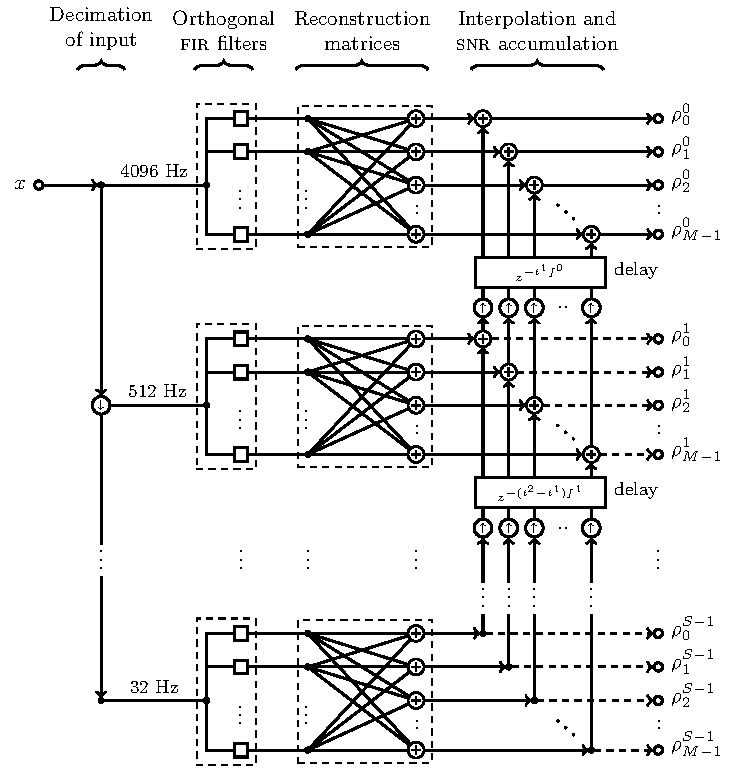
\includegraphics[width=\textwidth]{figures/lloid-diagram}
		\caption{\label{fig:pipeline} Schematic of \lloid{} algorithm.
		Circles with arrows represent interpolation
\protect
\includegraphics[scale=3]{figures/upsample-symbol} or decimation
\protect
\includegraphics[scale=3]{figures/downsample-symbol}.  Circles with plus
signs represent summing junctions
\protect
\includegraphics[scale=3]{figures/adder-symbol}.  Squares
\protect
\includegraphics[scale=3]{figures/fir-symbol} stand for \fir{} filters.  Sample
rate decreases from the top of the diagram to the bottom.}
	\end{center}
\end{figure}

\begin{equation*}
	\rho_i^s [k] =%
		% Interpolation SNR
		\color{diagramaccum}
		\overbrace{
			\left(H^\uparrow \rho_i^{s+1}\right)[k]
		}^\text{\clap{{\sc snr} from prev. time slices}}
		% Plus ...
		\;\;+\;\;
		% Reconstruction
		\color{diagramreconstruct}
		\underbrace{
			\sum_{l=0}^{L^s-1} v_{il}^s \sigma_l^s
		}_\text{\clap{reconstruction}}
		% Orthogonal FIR filter
		\color{diagramfir}
		\;\overbrace{
			\sum_{n=0}^{N^s-1} u_l^s[n] \color{black}x^s[k-n]
		}^\text{\clap{orthogonal {\sc fir} filters}} .
\end{equation*}

\section*{Results and conclusion}

\begin{table}
\caption{\label{table:flops}Cost and latency of the \TD\ method, the \FD\ method, and \lloid.}
\begin{center}
\begin{tabular}{lll}
\toprule
method & \flops\ & latency (s) \\
\midrule
time domain & $2.4\times10^{13}$ & $0$ \\
frequency domain & $2.6\times10^8$ & $2\times10^3$ \\
\lloid\ (theory) & $4.7\times10^8$ & $2\times10^{-3}$ \\
\lloid\ (prototype) & ----------- & $5$ \\
\bottomrule
\end{tabular}
\end{center}
\end{table}

\PARstart{\color{ink1!50!black}W}{\color{ink1!50!black}e have demonstrated} a computationally feasible filtering algorithm
for the rapid and even early-warning detection of \GW{}s emitted during the
coalescence of neutron stars and stellar-mass black holes.  It is one part
of a complicated analysis and observation strategy that will unfortunately
have other sources of latency. However, we hope that it will motivate
further work to reduce technical sources of \GW{} observation latency
and encourage the possibility of even more rapid \EM\ followup observations
to catch prompt emission in the advanced detector era.

\end{minipage}%
\hspace{0.05\textwidth}%
\begin{minipage}[t]{0.25\textwidth}

\section*{Implementation}

\PARstart{\color{ink1!50!black}A}{\color{ink1!50!black}ccuracy and latency} are critical parameters. Figures
\ref{fig:tmpltbank} and \ref{fig:time_slices}
depict the masses used for the test and the resulting time-slice design. The
\SVD{} tolerance is set to 0.9999, which guarantees a fractional \SNR{} loss
less than 0.003. Table~\ref{table:flops} in Results summarizes measurements of
latency for a fixed accuracy based on a \gstreamer{}-based prototype of the
\lloid{} algorithm.

\begin{figure}[h]
	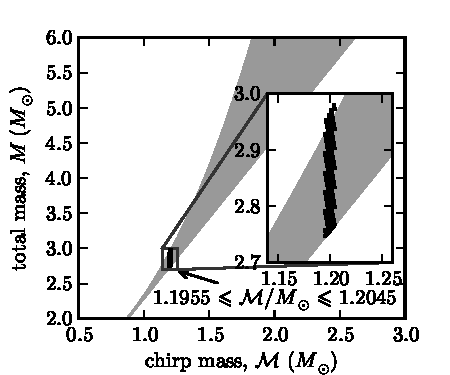
\includegraphics[width=1.1\textwidth]{figures/tmpltbank}
	\caption{\label{fig:tmpltbank}Source parameters selected for sub-bank used in this
case study.}
\end{figure}

\begin{figure}
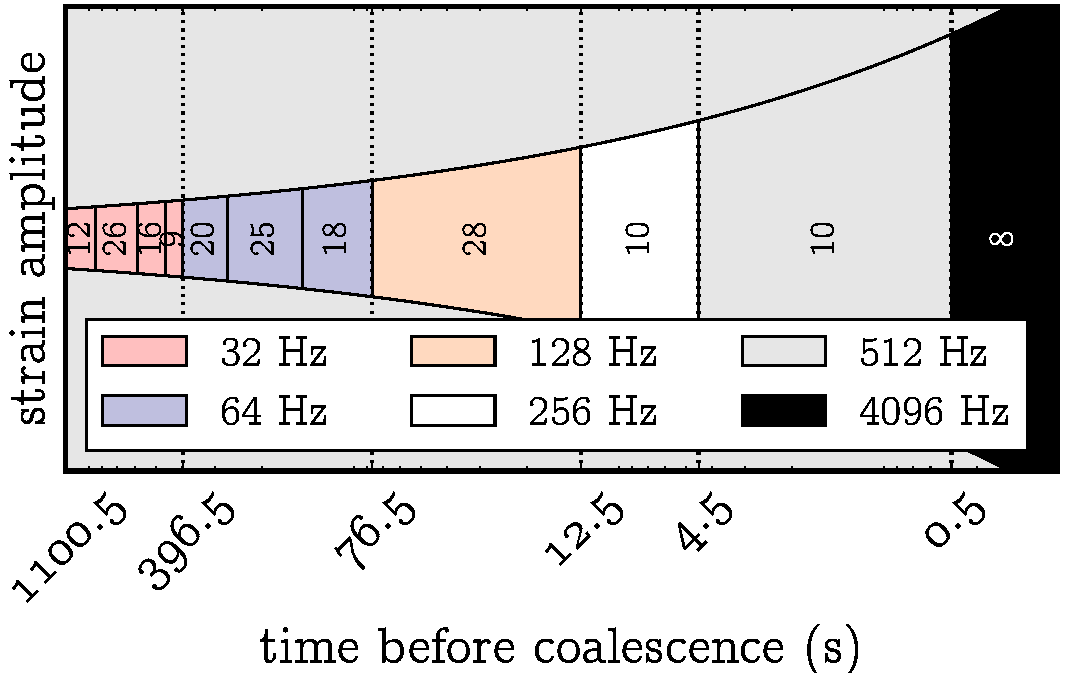
\includegraphics[width=\textwidth]{figures/envelope}
\caption{\label{fig:time_slices} Time slice parameters overlaid onto a representative waveform amplitude envelope.}
\end{figure}

\begin{figure}
\includegraphics[width=\textwidth]{figures/network}
\caption{\label{fig:gstreamer}Part of a typical GStreamer pipeline.}
\end{figure}

\end{minipage}

\begin{minipage}[t]{0.25\textwidth}
%%% References
\bibliographystyle{apj}
\bibliography{references}
\end{minipage}%
\hspace{0.05\textwidth}%
\begin{minipage}[t]{0.7\textwidth}
\section*{Acknowledgements}

This poster was prepared by \textsc{nf} and \textsc{ls} based on a preprint
article designated \LIGO{}-\textsc{p}\oldstylenums{0900004}. \LIGO\ was constructed by the California Institute of
Technology and Massachusetts Institute of Technology with funding from the
National Science Foundation (\textsc{nsf}) and operates under cooperative agreement
\textsc{phy}-\oldstylenums{0107417}. This research is supported by \textsc{nsf}
through a Graduate Research Fellowship to \textsc{ls}.


\includegraphics[height=3cm]{figures/LSC_logo}\hspace{7.5mm}
\raisebox{-7.5mm}{
\includegraphics[height=4.5cm]{figures/Caltech_logo}}\hspace{7.5mm}
\raisebox{-7.5mm}{
\includegraphics[height=4.5cm]{figures/nsf1}}
\raisebox{1.5mm}{\includegraphics[height=3cm]{figures/gstreamer-logo}}

\footnotesize{Amaldi 9, Cardiff, Wales, UK; This document bears the \textsc{dcc} number \LIGO{}-\textsc{g}\oldstylenums{1100683}-v\oldstylenums{1}.}

\end{minipage}

\end{document}
